\header{
    \section{Au 31 du mois d'Août} \label{au-31-du-mois-d-aout}
    %
    
    \insertComment{Chant traditionnel marin contant la bataille du 31 aout 1800 où la Confiance prit d'assaut le Kent, navire anglais comptant 38 cannons et 400 hommes.
    \\Lors de la prise du Kent, le dialogue suivant se serait déroulé entre les deux commandants :
    \\L'officier du Kent : "Nous, Anglais, nous nous battons pour l'honneur, et vous les Français, vous vous battez pour l'argent !"
    \\Robert Surcouf : "L'on se bat toujours pour ce que l'on n'a pas."
    }{Paru en 1859 dans "Chants et chansons populaires de la France Vol 2"}
}

\enluminure{4}{\href{https://www.youtube.com/watch?v=NZvNFHM0Axk}{A}}{u trente et un} du mois d'Août ~~~~~~~~ \bissimple
\\Nous vîmes venir sous l'vent à nous ~\bissimple
\\Une frégate d'Angleterre
\\Qui fendait la mer et les flots;
\\C'était pour attaquer Bordeaux.
\\\\\textbf{Refrain :}
\\Buvons un coup, lala
\\Tirons en deux, c'est mieux !
\\A la santé des amoureux, 
\\ A la santé du roi de France.
\\Et merd' pour le roi d'Angleterre 
\\Qui nous a déclaré la guerre.
\\\\Le capitaine du bâtiment ~~~~ \bissimple
\\Fit appeler son lieutenant : ~~ \bissimple
\\"Lieutenant, te sens-tu capable 
\\Dis-moi, te sens-tu assez fort
\\Pour prendre l'Anglais à son bord ?
\\\\Le lieutenant fier z'et hardi ~~~~~~~~ \bissimple
\\Lui répondit : "Capitaine, oui ! ~~ \bissimple
\\Faites Branle-bas à l'équipage,
\\Je vas hisser le pavillon
\\Qui rest'ra haut nous le jurons!" 
\\\\Le maître donne un coup de sifflet : ~~~~\bissimple
\\Carguez les voiles au perroquet, ~~~~~~~ \bissimple
\\Larguez les ris et vent arrière,
\\Laissez porter jusqu'à son bord,
\\Nous verrons bien qui s'ra le plus fort !"
\\\\Vire lof pour lof au même instant ~~~~~\bissimple
\\Nous l'attaquâmes par son avant ~~\bissimple
\\A coup de haches d'abordage
\\De sabres, de piques, de mousquetons,
\\Nous l'eûmes vite mis a la raison !
\\\\Que dira-t-on dudit bateau ~~~~~~~\bissimple
\\En Angleterre et à Bordeaux !! ~ \bissimple
\\De s'être ainsi laissé surprendre
\\Par un corsaire de six canons
\\Lui qu'en avait trente et si bons !
\dualcol{
\\\\\textbf{Refrain final :}
\\Buvons un coup, lala
\\Tirons en deux, c'est mieux !
\\A la santé des amoureux, 
\\A la santé des vins de France
\\A qui nous devons le succès
\\D'être vainqueurs sur les anglais !
\vspace{0.5cm}
\begin{center}
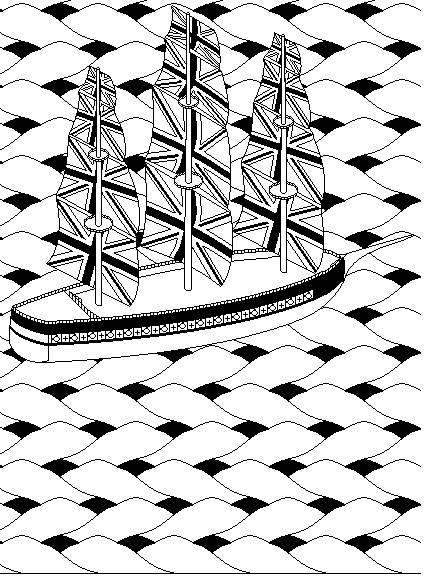
\includegraphics[width=0.5\textwidth]{images/31_mois_aout.jpg}
\end{center}
}

\breakpage